\chapter{Function evaluation}

The key purpose of the Scala Adaptive framework is to always invoke a function that is expected to have the best performance possible in given environment and with given inputs. By \textit{function performance} we mean any measurable description of the qualities of the function. It can be the actual runtime of the function, memory consumption, number of I/O operations, number of threads created, etc. All these factors can be valued and be the goal of the system run optimization.

This thesis is focused on the task of optimizing the function runtime or time complexity in general. The core of the framework, however, is designed to be extensible by modules that can analyze the function run in different ways. More on this topic will be covered in %TODO: REFERENCE

\section{Selection and invocation process}

Suppose we have a combined function \inlinecode{f()} created using the API described in chapter \ref{chapter:api} by combining multiple functions \inlinecode{f1()}, ..., \inlinecode{fn()}. We have a new function (or a function-like object) that can be invoked\footnote{In Scala terms applied} and we expect it to run one of the functions \inlinecode{f1()}, ..., \inlinecode{fn()}.

The basic steps required to do so are the following:

\begin{enumerate}
	\item Locate the runtime history data of \inlinecode{f1()}, ..., \inlinecode{fn()}
	\item Select the function \inlinecode{fk()} to be invoked
	\item Invoke \inlinecode{fk()} and evaluate its runtime
	\item Update the runtime history data of \inlinecode{fk()} with the new record
\end{enumerate}

\subsection{Runtime evaluation}

When talking about function runtime (or an execution time of a function), there are two types of values that we could be evaluating:

\begin{itemize}
	\item \textbf{\textit{Wall clock time}} - time elapsed between entering and leaving the function
	\item \textbf{\textit{CPU time}} - time that the CPU actually spent executing our function
\end{itemize}

The \textit{wall clock time} is always higher than the \textit{CPU time}, because it includes not only the time when CPU is executing the function code, but also the time when the executing thread is waiting for its turn in time-sharing multitasking OS or sleeping on a blocking I/O\footnote{Input / Output operation} operation, synchronization primitive, or for some other reason. This means that the \textit{wall clock time} also gets affected by concurrently running processes, network load, and other environment-based factors, and tends to vary much more between multiple invocations.

For the purposes of the ScalaAdaptive framework, it might seem that the \textit{CPU time} would be more appropriate, as it gives clearer results not affected by the state of the executing environment. The truth is, however, that many of the use cases of the framework require the thread sleeping time to be included in the measurement, as the functions runtimes are determined mainly by the duration of an I/O operation (e.g. database queries, network requests, etc.), so using \textit{CPU time} wouldn't give us the necessary results.

It is also quite difficult to determine the \textit{CPU time} - it requires support from the executing system with tracking the time that every thread has spent in execution. For this reason and for the reason stated above, the selection process in this text is based on \textit{wall clock time}. It might be, however, interesting as a future extension to implement measuring both of the times and allowing the user to select for each combined function which time should be measured.

The \textit{wall clock time} is measured by fetching high-precision system time in nanoseconds right before calling the function apply method and right after returning from the call. The result is the runtime in nanoseconds. This measurement is precise enough for all the use cases of the framework, because it's targeting functions with non-negligible time complexities.

\subsection{Storing the evaluation data}

After having invoked the function and evaluated its runtime, the evaluation data have to be stored before passing the return value back to the caller. Multiple types of storage can be used for that.


\section{Selection strategies}
\label{sec:selection_strategies}

The most complicated task of the entire chain is to select the most appropriate function to run in given case. The case is described by an input \inlinecode{in} of the function \inlinecode{f()} and by the evaluation data gathered in previous runs.

The most straightforward approach would be to look at the function run history and select the function with the lowest average runtime in the measured runs. This solution has a few problems. First of all, the runtime of the inner functions \inlinecode{f1()}, ..., \inlinecode{fn()} might depend on the input \inlinecode{in}, which could lead to incorrect assumptions if the historical data were measured on runs with various inputs. And secondly, the method doesn't solve the case where the data don't give us an exact answer, for example if there are too few, if the historical results are too scattered (which might have been caused by different conditions upon invocation, etc.), and in general when we can't make a clear decision and need to collect more data instead.

The \textit{input dependency} problem might be solved in various ways. Methods to analyze the relation between the input and the runtime might be employed in order to predict an approximate runtime on a new input. We call these methods \textit{predictive strategies}. A simpler approach that can be used universally with any \textit{non-predictive strategy} without changing it dramatically is to apply it on a smaller subset of the history records that have inputs of a very similar size. 

As for the \textit{uncertainty} problem, the key is to collect a fixed amount of data first before using any of the strategies. Additionally, a techniques from statistical testing can be used so that the strategy could have a maximal probability of an error (a wrong decision).

Based on these observations, a couple of strategies to select function were proposed and implemented as a part of the ScalaAdaptive framework. The user of the framework can decide by himself on which one to use.

\subsection{Predictive strategies}

These strategies are useful solely for the purpose of the functions for which the runtime is directly related to the input of the function, e.g. size of a data structure, length of a data file, a number, etc. The computational complexity of algorithms is usually expressed as a function of the size of the algorithm's input. The actual runtime depends on the complexity, as every computational step has to take some CPU time. 

The problem is that in reality, the duration of different steps differ as well, depend on hardware optimization, cache misses, pagefaults, scheduling of the OS and many other factors, so the relation, although still present, gets very distorted. For the purposes of only approximate predictions in order to determine faster function, we will suppose that for function \inlinecode{f()} \(\exists g\) so that 
\(\forall in\) possible inputs holds \(t = g(in)\), where \(t\) is the runtime on input \(in\) of \inlinecode{f()}.

The input, as mentioned earlier, can be a complex structure with a lot of factors contributing to the runtime\footnote{Consider for example a general graph - for most of the algorithms, both number of vertices and edges have to be taken into account}. For the simplicity of the strategies, we need to introduce an \textit{input descriptor} - an integer that can be computed from the input and that can be used as an input for the function approximation. In other words, we suppose that for function \inlinecode{f()} \(\exists h, g_1\) so that
\(g = h \circ g_1\) 
and 
\(\forall in \quad h(in) \in \mathbb{N}\). In this case, the \textit{input descriptor} of input \(in\) would be the value of \(h(in)\).
This assumption is not true in general, but in most cases, a sufficient function \(h\) can be found so that the results will be precise enough. We call it the \textit{descriptor function}

The \textit{descriptor function} has to be provided by the user of the framework. %TODO: reference to API?
Such function could be:
\begin{itemize}
	\item Number of elements in a data structure argument
	\item Sum of numbers of vertices and edges in a graph
	\item Size of a data file
	\item Identity, if the input is an integer determining the complexity (such as factorial, Fibonacci sequence, etc.)
\end{itemize}
Naturally, the \textit{descriptor function} itself shouldn't have a significant complexity, as it is going to be invoked during every call.

The task of the strategies listed in this section is to make an approximation of the \(g_1\) function and use it to compute \(g_1(h(in))\) upon every invocation and to select the function with the best (minimal) result.

\subsubsection{Simple linear regression}
\label{subsubsec:simple_linear_regression}

First strategy supposes that the function \(h\) can be approximated precisely enough using a linear function \(h'\) in the following form:
\[h'(x) = a' x + b'\].

This approximation is a \textit{simple linear regression model}. The slope \(a'\) and intercept \(b'\) of the linear function can be determined using a least squares method, which minimizes the squares of the distances of the actual function values from the ones predicted by the model.

A big advantage of the model is its simplicity and thus minimal overhead when generating the regression during the selection process. 

The main problem is that the linear regression model applied to a case where the relation is not linear leads to a non-trivial errors that increase with the range that we're trying to cover with the model. Figure \ref{fig:selection_sort_linear_trendline} shows samples of run times of the basic selection sort algorithm, which has the complexity of \(O(N^2)\), on sample arrays with 0 to 30000 integers. Collected data obviously match the quadratic function graph marked with the green color. The red line shows the linear regression model. As we can see, the predictions based on this model would be quite inaccurate, especially if we tried to predict run time on an input significantly larger than the samples.

\begin{figure}[h!]
	\centerline{\mbox{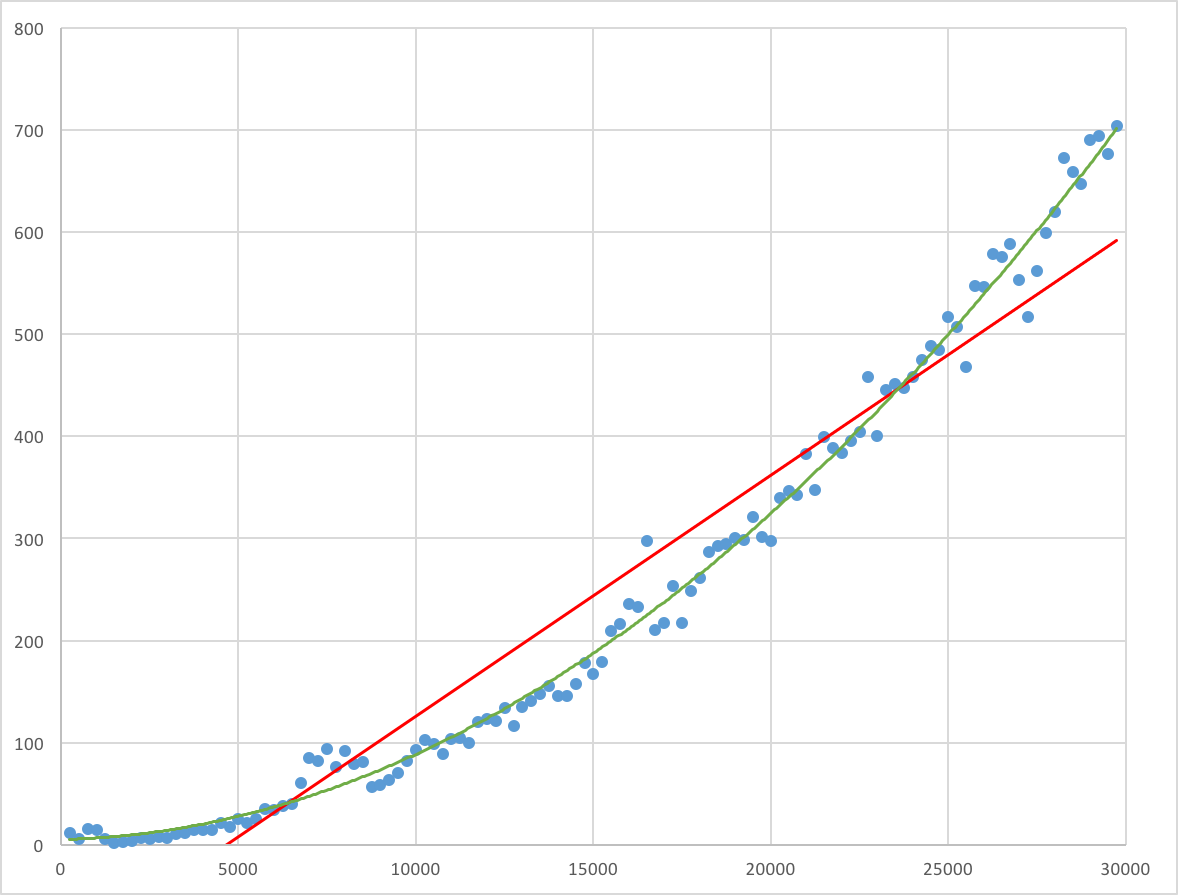
\includegraphics[width=90mm]{./img/selection_sort_linear_trendline.png}}}
	\caption{Linear regression line (red) of a selection sort runtime samples.}
	\label{fig:selection_sort_linear_trendline}
\end{figure}

In order to ensure the accuracy of the model, we can perform statistical tests on it. We can test the true slope \(a\) of the hypothetical original linear function, against a constant value \(a_0\). Suppose we have a linear regression model \(h'(x) = a' x + b'\) constructed using \(n\) data samples \(x_i, y_i\) (in our case, \(x_i\) are the input descriptors and \(y_i\) are the run times). The hypotheses would be the following:

\[H_0: a = a_0 \]

\[H_1: a \neq a_0 \]

The test statistics \(T\) for the test can be computed using the following formula:

\[T = \frac{a' - a_0}{se(a')}\]

where

\[se(a') = \sqrt{\frac{\sqrt{MSE}}{ \sqrt{ \sum_{i = 1}^{n} (x_i - \bar{x})^2 }}} \]

and

\[MSE = { \sum_{i = 1}^{n} (y_i - y_i')^2 }\]

The \(\bar{x}\) is the average of \(x_i\) and \(y_i' = h'(x_i)\).

Now, the \(T\) follows a \textit{t-distribution} with \(n-2\) degrees of freedom, so \(H_0\) is rejected on the significance level $\alpha$ in favor of $H_1$ in the following case:

\[\abs{T} > t_{n - 2}(1-\frac{\alpha}{2})\]

The $t_{n - 2}(1-\frac{\alpha}{2})$ is the $(1-\frac{\alpha}{2})$-th quantile of \textit{t-distribution} with $n-2$ degrees of freedom.

In our case, we have no specific $a_0$ that we want to test against, we simply want to know, if the data measured have a linear relation. We can achieve this by putting $a_0 = 0$. If we reject $H_0$ on the significance level $\alpha$, there is a $1 - \alpha$ probability of the data having a linear relation, and in such a situation, we can use the $a'$ slope of the simple linear regression model without too many issues.

\begin{figure}[h!]
	\centerline{\mbox{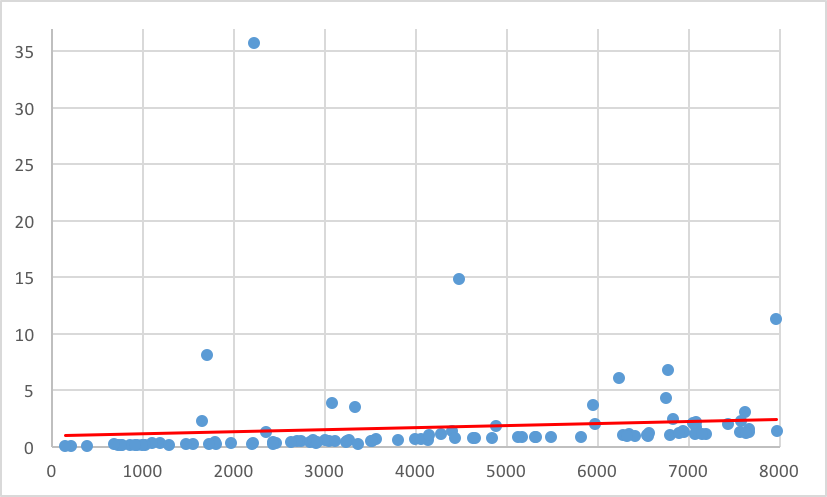
\includegraphics[width=90mm]{./img/linear_cantreject.png}}}
	\caption{Linear regression of 100 run time samples from a function with linear complexity where $H_0$ couldn't be rejected.}
	\label{fig:linear_cantreject}
\end{figure}

Unfortunately, the test tends to get affected by random fluctuations in function run times, which are quite common, especially for simple functions with short execution. The figure \ref{fig:linear_cantreject} shows a regression performed on a sample of 100 run times of a function with linear complexity. The slope of the linear approximation seems to match the measured data reasonably well, but the hypothesis $H_0$ of the statistical test couldn't be rejected on the significance level $\alpha = 0.05$. 

On the other hand, figure \ref{fig:quadratic_rejected} shows a regression performed on a sample of 100 run times of a function with quadratic complexity, and in this case, the hypothesis $H_0$ of the was rejected in favor of $H_1$ on the same significance level $\alpha = 0.05$.

\begin{figure}[h!]
	\centerline{\mbox{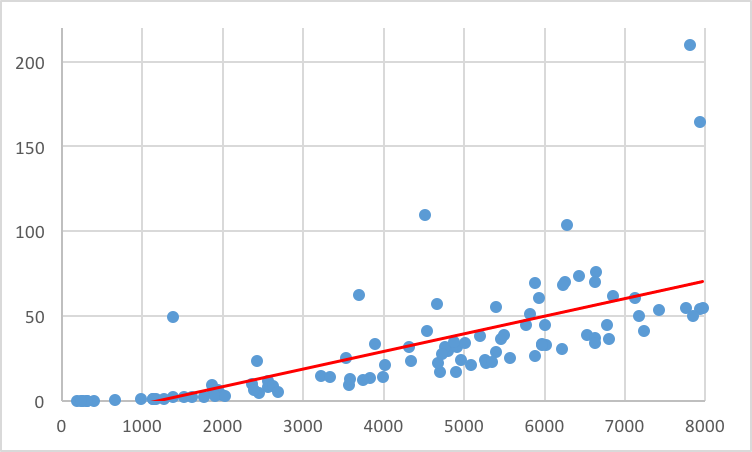
\includegraphics[width=90mm]{./img/quadratic_rejected.png}}}
	\caption{Linear regression of 100 run time samples from a function with quadratic complexity where $H_0$ was rejected.}
	\label{fig:quadratic_rejected}
\end{figure}

\subsubsection{Window-bound linear regression}
\label{subsubsec:window_bound_regression}

Tobe able to apply the strategy described in section \ref{subsubsec:simple_linear_regression} on a wider range of functions, a simple approach to lower the approximation errors can be taken. Instead of creating a regression model for the entire set of measurements at once, we can split it into more subsets and create different regressions for them. Figure \ref{fig:window_examples} shows ranges $5000 - 10000$, $10000-15000$ and $15000-20000$ for the input sizes of the data from \ref{fig:selection_sort_linear_trendline}. As we can observe from the second and third range, the data tend to be much closer to the linear regression line. The first range shows that a less significant fluctuation in the entire set has a lot bigger impact on a smaller subset.

\begin{figure}[h!]
	\centerline{\mbox{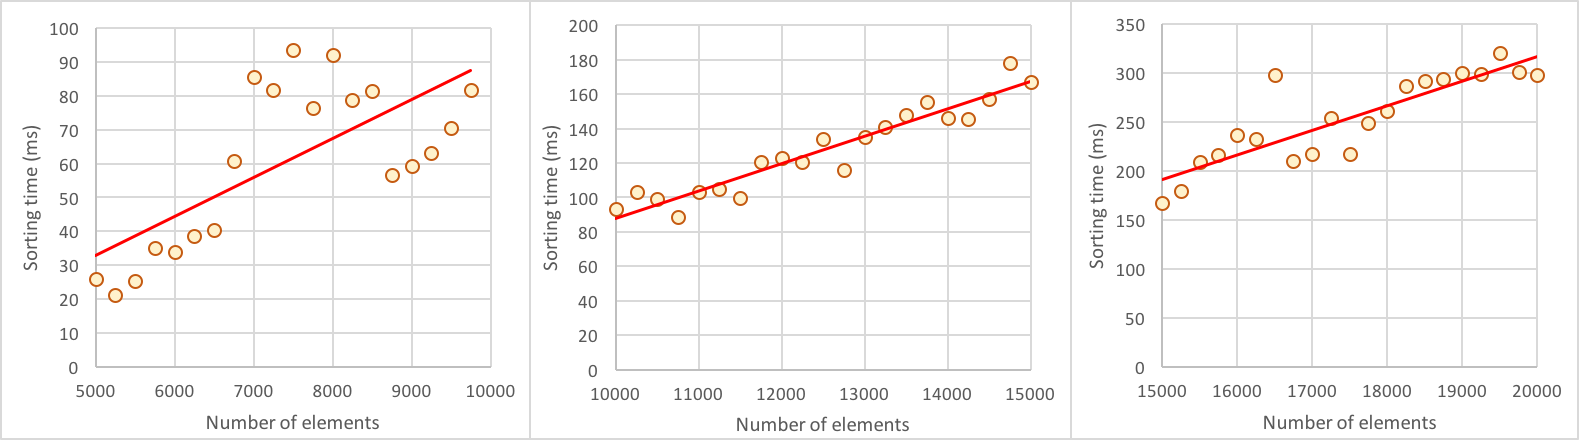
\includegraphics[width=110mm]{./img/window_examples.png}}}
	\caption{Examples of subsets of the data from figure \ref{fig:selection_sort_linear_trendline} with linear regressions.}
	\label{fig:window_examples}
\end{figure}

When selecting a function for a specific \textit{input descriptor} $desc$, a window around its value of specific width $w$ can be selected and the regression model built upon it. We do it by selecting the data samples $x_k, y_k$ where $\abs{x_k - desc} < w$, and using them as the entire data set.

The window width $w$ can be selected in multiple ways. Using a fixed number across all the functions and all the data samples wouldn't be recommendable, as the functions can vary in their \textit{input descriptors} by orders of magnitude. The width could be derived as a fraction of the width of the whole data set: $w = \frac{max(x_i) - min(x_i)}{p}$, where $p$ would represent in how many parts we basically want to split the set. This wouldn't help us in a case where there are a few extreme values of \textit{input descriptors} in the data set and the rest of the values lies together. 

The most complicated but also the most adaptive window selection method is based on analysis of the entire data set - we sort the samples using the \textit{input descriptor} and compute the distances of each pair of the neighboring ones, make an average of these distances and set the $w$ as $avg * m$, where m is the expected number of samples in one window. For the value of $m$, we can chose a number of about $50-100$.

\subsubsection{Local regression}

The approach explained in \ref{subsubsec:window_bound_regression} can be extended further - the locally constructed linear regression models can be used to build up a model for the entire data set. This leads to a model that is non-linear, in other words, the function that approximates the original data relation is not a linear function.

One possible regression method that behaves this way is \textit{LOESS} (Local Regression). It uses methods similar to the least-square regression on local subsets of the data set, and then smooths up the resulting curve. The result is a \textit{Loess Curve}, which is a function that is artificially constructed and doesn't have any simple (or even known) formula. This is the one of the advantages - the original relation between \textit{input descriptors} and the run times didn't have to be expressed by a nice simple function in order to be modeled correctly.

%TODO: Add some sources

There is also a few disadvantages of this strategy. First of all, the entire local regression model has to be recomputed whenever there is a new data in the dataset, the model can't be simply updated like the \textit{simple linear regression}. Secondly, it is much more computationally complicated and the model construction takes non-trivial time, so it has a negative impact of the framework overhead, especially when used with short and simple functions. Next, there is no simple way how to perform statistical tests on the accuracy of the model. The last downside of \textit{local regression} is its inability to predict further behavior past the minimum and maximum data sample.

\subsubsection{Whitebox model construction}

The methods that were described so far are examples of the blackbox techniques - they don't analyze the function itself, they base all their predictions only on the runtime measured.

More thorough predictions could be made after examining the function code as well. It can be analyzed, key structures in the code identified (loops, branches, function calls, variables) and a model can be created using these information. The code can be instrumented and the measurement can be done for each of the structures mentioned. It would require more complex runtime measurement data, but the framework is prepared for this. The prediction will then be based on the model and the data measured for its elements.

%TODO: Add reference / bibliography
Similar approach was taken in [Predicting Execution Time of Computer Programs] with the goal of predicting program execution time on a specified input with very high precision.
%TODO: Add results?

This approach has a few problems concerning the intended use cases of ScalaAdaptive framework. The model won't add any value to the predictions if the majority of the execution time will be spent waiting on an I/O operation. Specifically, it won't help with any of the cases where we are selecting a database query, remote server to connect to, etc.

For these reasons and because of the complexity, it wasn't implemented in the framework, but it represents a potential future work that could be done on the topic.

\subsection{Comparison of predictive strategies}

\subsection{Non-predictive strategies}

In some cases, the function run time doesn't depend on the input, or the relation isn't significant enough. In such a case, we consider all the runs of the function equal and we want to decide based on the historical measurements which one of the functions has a higher chance of being faster.

The trivial solutions being the following:
\begin{itemize}
	\item Select the function with the lowest average run time
	\item Select the function with the lowest minimal runtime
	\item Select the function with the lowest maximal runtime
\end{itemize}

Each of these strategies does make sense and might be useful in some cases, the problem is that they can't give us the certainty with which the function is better. Again, using statistical methods to express the level of certainty we require from the decision, can solve the problem.

\subsubsection{T-test for two functions}

If we assume that the measured function run times come from a normal distribution, we can use the methods of statistical testing to determine whether one function is faster than the other with given significance. 

Suppose we have two samples of run times for the two functions involved, $X_1, ..., X_n$ and $Y_1, ..., Y_m$. Next, suppose that these samples come from normal distributions with expectations $\mu_1$ and $\mu_2$, respectively. These expectations are unknown for as, just like the variances. The goal is to test the expectations of the two samples against each other. 

Based on these requirements, we will use a \textit{two-sample t-test}. The default hypotheses for the test are:

\[
H_0: \mu_1 = \mu_2
\]
\[
H_1: \mu_1 \ne  \mu_2
\]

and the test statistics

\[
T = \sqrt{\frac{nm}{n + m}}\frac{\bar{X}_n + \bar{Y}_m}{S}
\]

where $\bar{X}_n$ and $\bar{Y}_m$ are the sample averages and $S$ is the common variance estimate computed as a weighed average of the sample variances:

\[
S^2 = \frac{1}{n + m -2} ((n-1)S_X^2 + (m-1)S_Y^2)
\]

with $S_X^2$ and $S_Y^2$ being the sample variances:

\[
S_X^2 = \frac{1}{n-1} \sum_{i=1}^{n}(X_i - \bar{X}_n)^2
\]
\[
S_Y^2 = \frac{1}{m-1} \sum_{i=1}^{m}(Y_i - \bar{Y}_m)^2
\]

The hypothesis $H_0$ will be rejected in favor of hypothesis $H_1$ with the significance level $\alpha$ if

\[\abs{T} > t_{n + m - 2}(1-\frac{\alpha}{2})\]

The $t_{n + m - 2}(1-\frac{\alpha}{2})$ is the $(1-\frac{\alpha}{2})$-th quantile of \textit{t-distribution} with $n+m-2$ degrees of freedom.

Rejecting $H_0$ in favor of $H_1$ means that the sample distributions have significantly different expectations, i.e., one of the functions is expected to give better results than the other. In order to find out which of the functions is the favored one, we need to use a \textit{one-sided test}. To do so, we introduce additional hypotheses:

\[
H_2: \mu_1 > \mu_2
\]
\[
H_3: \mu_1 < \mu_2
\]

Now we can reject the hypothesis $H_0$ in favor of $H_2$ if

\[T > t_{n + m - 2}(1-\alpha)\]

or reject the hypothesis $H_0$ in favor of $H_3$ if

\[T < -t_{n + m - 2}(1-\alpha)\]

By performing the \textit{one-sided tests} with $H_2$ and $H_3$ as alternatives, we can easily determine, which of the functions has lower expectation of run time and is a candidate to be selected to run.

\subsubsection{T-test for multiple functions}

\section{Grouping}

\section{Selection policies}

The selection process and all the strategies described in \ref{sec:selection_strategies} are quite complex and have non-trivial overhead, especially after collecting a large amount of historical data. In a common scenario where we expect the system to come to a decision about the best function (either overall, or for every group of \textit{input descriptors}), it would be handy if we could stop the selection process at a certain point and keep using only the most favored function with no extra overhead. Or, to use it most of the time, with only occasional attempts at the selection in order to detect possible changes in the system (response times, I/O operation duration, etc.).

Similarly, it might be desirable to control the overhead time spent on the selection, or, in general, on invoking the functions using selection (which might lead to a bad decision), either per a specific time period, or per a specific action of the system (user request, processing unit, etc.). All of these decisions are taken at a higher level than the run time history analysis performed by the selection strategies.  

\textit{Selection policies} are a concept introduced into the ScalaAdaptive framework that tries to address these cases, with the main purpose of lowering its execution overhead. Every \textit{combined function} has a \textit{selection policy} associated with it. In the function selection chain, the \textit{policy} gets evaluated right after invoking the function and is supposed to quickly decide how to proceed with the invocation. There might be scenarios where a faster ways could be taken without even using any of the strategies and analyzing the historical data.

The possible results of the \textit{policy} evaluation are the following:

\begin{itemize}
	\item \textbf{SelectNew} - Select function using the selection strategy
	\item \textbf{GatherData} - Gather more data for the least-executed function
	\item \textbf{UseLast} - Use the function selected last time
	\item \textbf{UseMost} - Use the most selected function
\end{itemize}

We can notice that these results require only the basic statistical data about previous selection processes. This is the key idea of the \textit{policies} - the decision and the execution should depend only on these simple statistics, except for the case where selection strategy is required.

The \textit{policy} evaluation process also replaces the current \textit{policy} with a new one. This technically creates a state machine - the state of the function is represented by the active \textit{policy}, and whenever the function is invoked, a result is produced and new \textit{policy} becomes active. This corresponds to producing output and moving to a new state in a state machine.

The advantage of the \textit{policy} system over a regular state machine is its extensibility and reusability - there are no rules directly in the state machine (i.e. here in the \textit{combined function}). All the logic of deciding on the result and the next \textit{policy} is in the \textit{policy} node itself. So the entire behavior of the state machine is defined by the initial \textit{policy}, which is specified by the user upon creating the \textit{combined function}. As a result, reusable policies that are parametrized can be used in various chains of policies, smaller chains can be put together, etc.
%TODO: Reference to the API

\subsection{Statistical data}

The only input that the \textit{policy} receives when making decision is a statistical summary of previous selection results of the \textit{combined function}. The process itself is supposed to be fast and reflect just the trends in the selection, not to replace the whole selection strategy process as described in section \ref{sec:selection_strategies}, so the statistical data don't contain the entire run history of all the functions involved.

\begin{figure}[h!]
	\centerline{\mbox{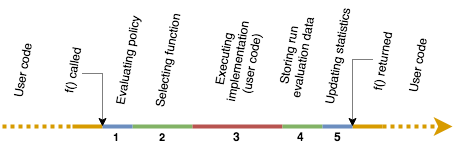
\includegraphics[width=110mm]{./img/run_schema.png}}}
	\caption{Process of \textit{combined function} invocation.}
	\label{fig:run_schema}
\end{figure}

On the other hand, the \textit{policies} are a handy tool to limit the damage of the selection process on the system. For this, it is necessary to observe and to store various times connected with the selection and execution. Figure \ref{fig:run_schema} shows the whole process with policy being evaluated with the SelectNew result, split into individual parts. Upon every invocation, the following is tracked:

\begin{itemize}
	\item Selection and run history storage time (2 and 4)
	\item Function execution time (3)
	\item Total time spent on the SelectNew result (2, 3 and 4)
\end{itemize}

These times are added up to a sum for every function after every SelectNew result. In addition, the total time spent on running the lest-executed function is tracked when GatherData result is received, and also added up. The policy can work with these totals and analyze the changes that happen to them overtime. The policies are designed to be immutable, but contain state themselves, and the state changes when switching to a new policy.

In addition, number of times each function was selected, total number of times we received the SelectNew and GatherData result and the total number of times the combined function was invoked has to be tracked. The user-implemented policy has the following data available to decide:

\begin{itemize}
	\item Total run count of the combined function
	\item Total number of times the last function was selected
	\item Total number of times the most selected function was selected
	\item Total number of times any function was selected
	\item Total number of times of gathering new data (GatherData result)
	\item Total time spent on function execution (after SelectNew result)
	\item Total time spent on selection and storage overhead (after SelectNew result)
	\item Total time spent on processing the SelectNew result
	\item Total time spent on processing the GatherData result
\end{itemize}

\subsection{Implemented policies}

A simple description of policies that were implemented as part of the framework and used in its evaluation follows. Note that it is very simple to create own customized policies and the topic will be covered later.



\subsection{Possible improvements}

Part of the statistical data could be a factor of combined certainty of all the selections of a specific function. This factor could be combined from the selection results of the strategies that would support it (in the statistical test based strategies, it could be a p-value, strength of the test, or similar) and would serve as a decision factor for more complex policies with a statistical approach as well.

%TODO - when do I need more data?